\section{Introduction}
\label{sec:intro}

The age of {\large big data} is upon us as organizations large and small 
are coping with massive volumes of data from sensors, website 
clicks, e-commerce, and more. In recent years, there has been 
growing interest in developing frameworks for the storage and 
analysis of this data on large compute clusters, 
Hadoop~\cite{CuttingCa05,DeanGh08} being among among the most 
popular of these. Hadoop breaks up 
large datasets into pieces distributed across many shared-memory
multi-core nodes in a cluster, each of which communicates via
a message-based network protocol. Users supply computations, 
or \defn{map} operators, that are evaluated over each of 
the pieces independently and other computations, or \defn{reduce} 
operators, that combine the results. 
Many problems can be cast into the Hadoop model, but in many 
cases the Hadoop approach is far less effecient than more 
specialized methods, as we will explore throughout this paper.

The idea behind recent big data frameworks, including Hadoop, 
is to decouple scheduling and
data layout from the expression of the computation, enabling high
programmer productivity and portable, best-in-class performance.
However, iterative graph algorithms are one class of problems that
is not well-suited to the Hadoop approach. In particular, each 
Hadoop computation writes its output to disk, so each iteration 
in iterative computations incurs the overhead of a disk write 
and then a subsequent disk read for the next iteration. In 
addition, graphs are difficult to split into completely 
independent sets (with no crossing edges) for the map phase 
of a Hadoop computation, so the maps are often wasteful.
However, the idea of decoupling data and scheduling from the expression of
the algorithm is very useful for designing frameworks
for graph algorithms, even if Hadoop itself is ill-suited to 
the task.  
%Functional programming - more copying
%Fault tolerance - not valued in physical simulation space


\subheading{Motivation and Problem Definition}

This paper investigates the problem of performing physical simulations
expressed in the language Simit on very large datasets quickly and
deterministically.  Simit generates a static graph, as in \figref{mesh}, 
which is typically
locally connected and embeddable in a $N$-dimensional space, where typically
$N=3$.  Then, a function that operates on each vertex and its neighbors 
is applied to all vertices over many (e.g. at least millions) time steps.
These functions are typically some approximation of physical forces (e.g.
Newton's laws)  

\begin{figure}[h]
\centering
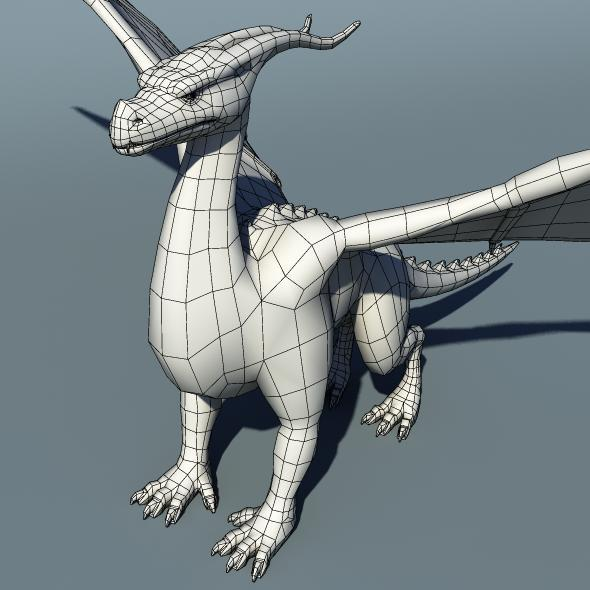
\includegraphics[width=2.5in]{dragon}
\caption{A mesh graph where lines correspond to edges and intersections of lines correspond to vertices.}
\label{fig:mesh}
\end{figure}




\subsection{Data-graph Computations}
		\begin{itemize}
		\item Definition
		\item Scheduling algorithms
		\item Qualitative rationale for cache perils of chromatic and potential benefit to dag scheduling
		\end{itemize}

In response to these shortcomings of Hadoop and similar systems, 
Guestrin et al developed the GraphLab 
framework~\cite{LowBiGo12} for iterative graph algorithms. 
The computation model here associates data with each node in a 
graph, and in each iteration runs an update function on each 
node that takes as input the data of the node and that of its 
neighbors. A node can only be updated for the $n$th time if 
its neighbors have been updated either $n-1$ or $n$ times. 
Many interesting big data algorithms, including Google's 
PageRank, can be easily expressed under this model. GraphLab 
comes in two variants -- a single-machine implementation that 
attains parallelism by updating nodes concurrently on multiple 
processing cores, and a distributed implementation that 
additionally spreads vertices across machines.



\begin{figure}[h]
\centering
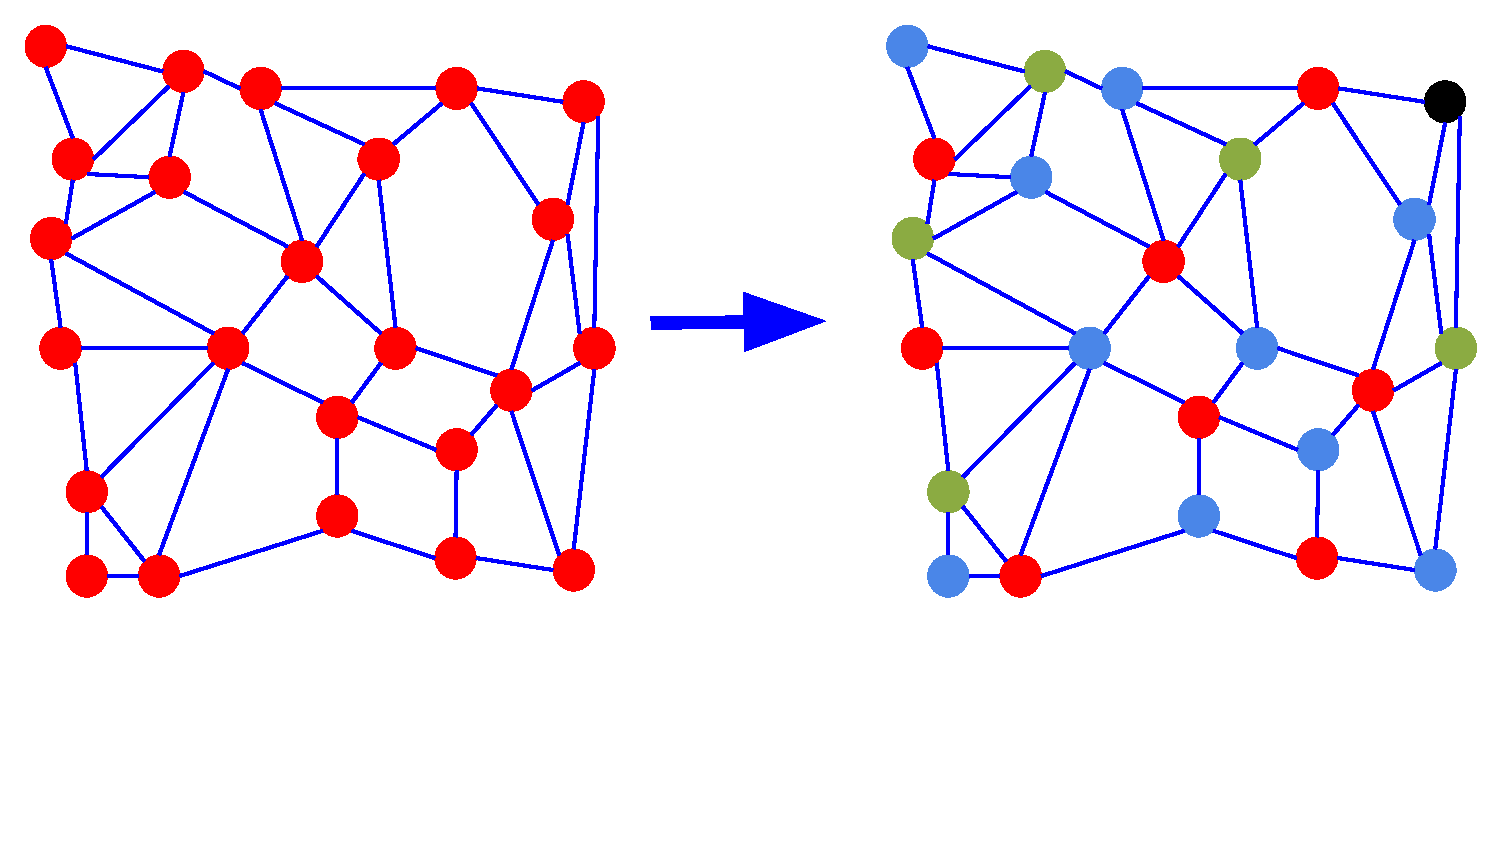
\includegraphics[width=5in,clip,trim=0 3cm 0 0]{chromatic_scheduling.pdf}
\caption{Example of how a graph can be partitioned into 
independent sets of vertices denoted by color, each set of which is able to
be executed simultaneously without causing data races.  Iterating
through the colors serially and executing the corresponding
independent sets in parallel is a technique called \emph{chromatic scheduling}.}
\label{fig:}
\end{figure}

As GraphLab and competing frameworks have become more popular, 
there has been growing interest in optimizing their execution. 
In the single-machine case, there has been work on reducing 
costly sychronization steps and more generally on increasing 
parallelism so that performance can scale up as core counts 
grow. In the distributed case, the single-machine optimizations 
have been supplemented by work on more effectively splitting up 
nodes into sets with few crossing edges so that expensive 
inter-machine communication can be reduced.

\begin{figure}[h]
\centering
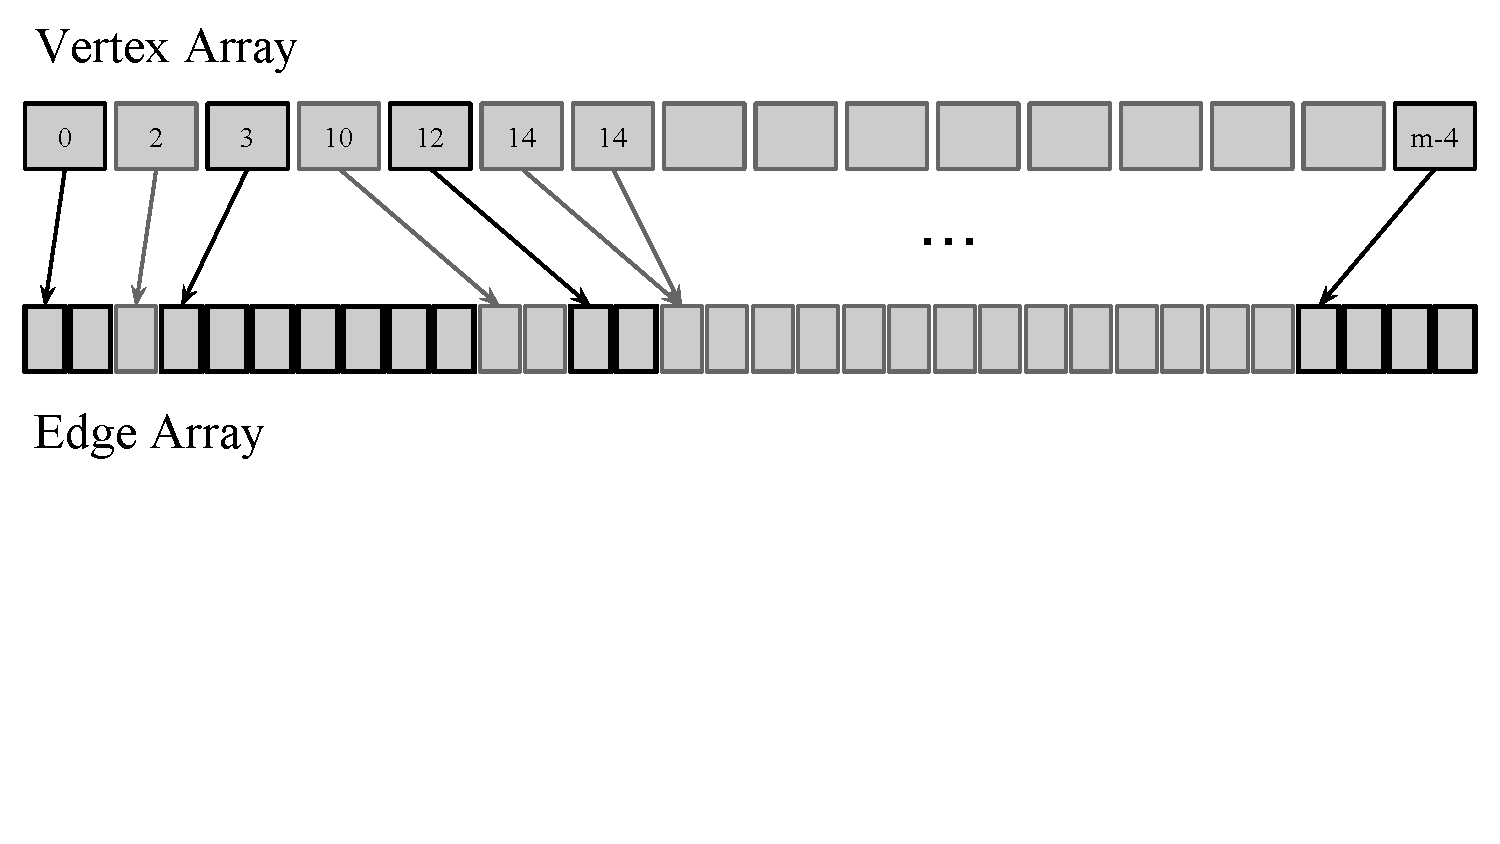
\includegraphics[keepaspectratio,width=4.5in,clip,trim=0 5cm 0 0]{sparse_matrix_representation.pdf}
\caption{Graphs are stored in memory on a single cache-coherent
multi-core in a sparse-matrix format.  The vertex array contains
vertex data and an index into an edge array, which contains vertex
IDs of the associated neighbors.}
\label{fig_layout}
\end{figure}


\begin{figure}[h]
\centering
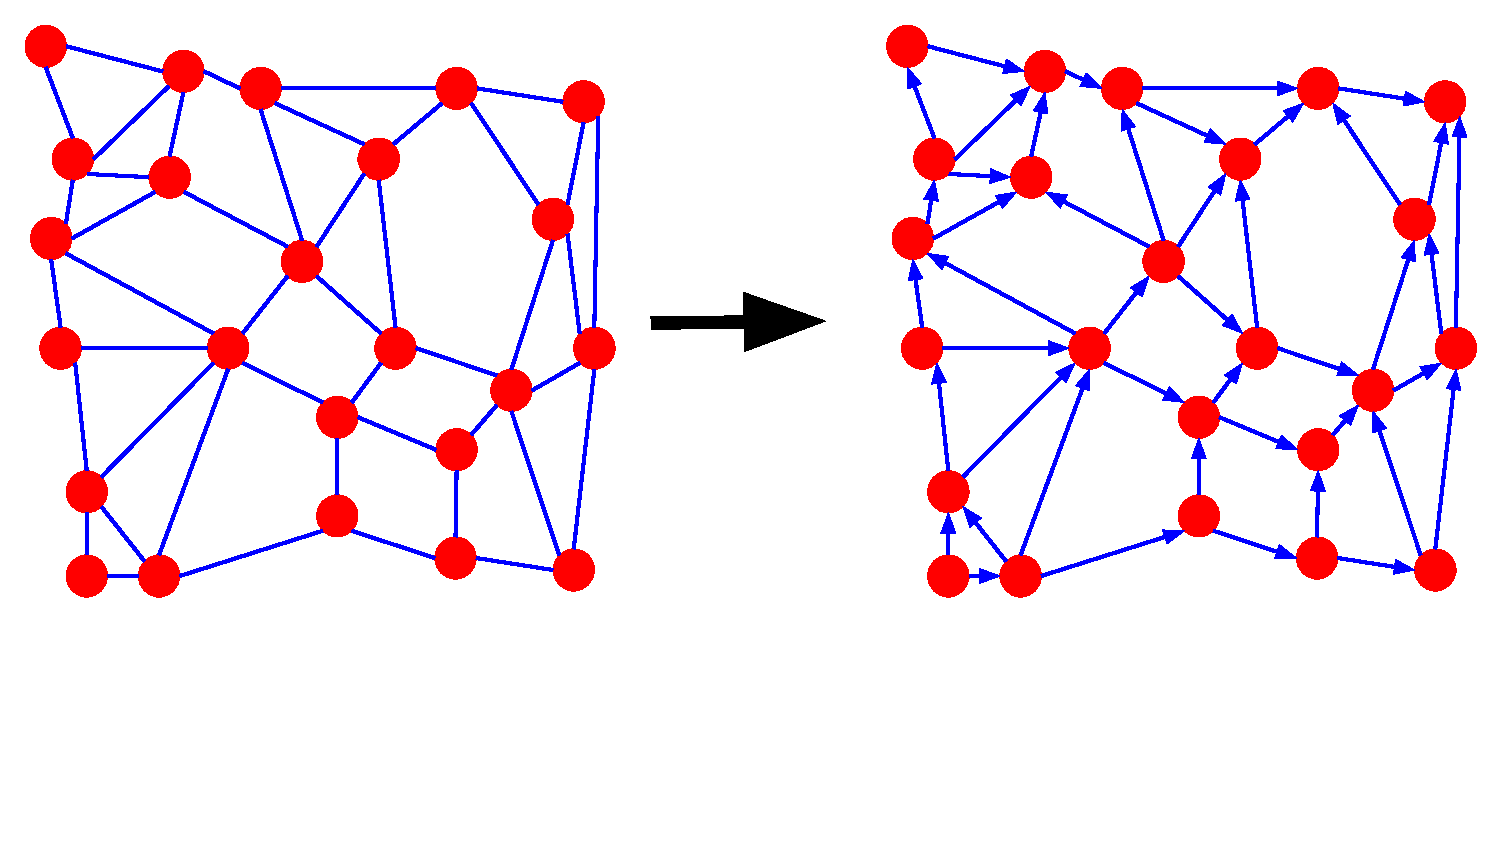
\includegraphics[width=5in,clip,trim=0 3cm 0 0]{dag_scheduling.pdf}
\caption{An alternative to chromatic scheduling, which 
yields a deterministic, data race-free output, is dag scheduling.
A priority funcrtion $\rho : V \rightarrow \mathbb{R}$ is used
to create a partial order on the vertices, orienting an edge from
low to high priority results in a 
dag.  The vertices are processed in dag order: a vertex is not
processed until all of its predecessors have been processed.}
\label{fig:}
\end{figure}




\subsection{\proc{Simit}}
		\begin{itemize}
		\item High-level description
		\item How to represent graph as a DGC
		\end{itemize}


\begin{figure}[h]
\centering
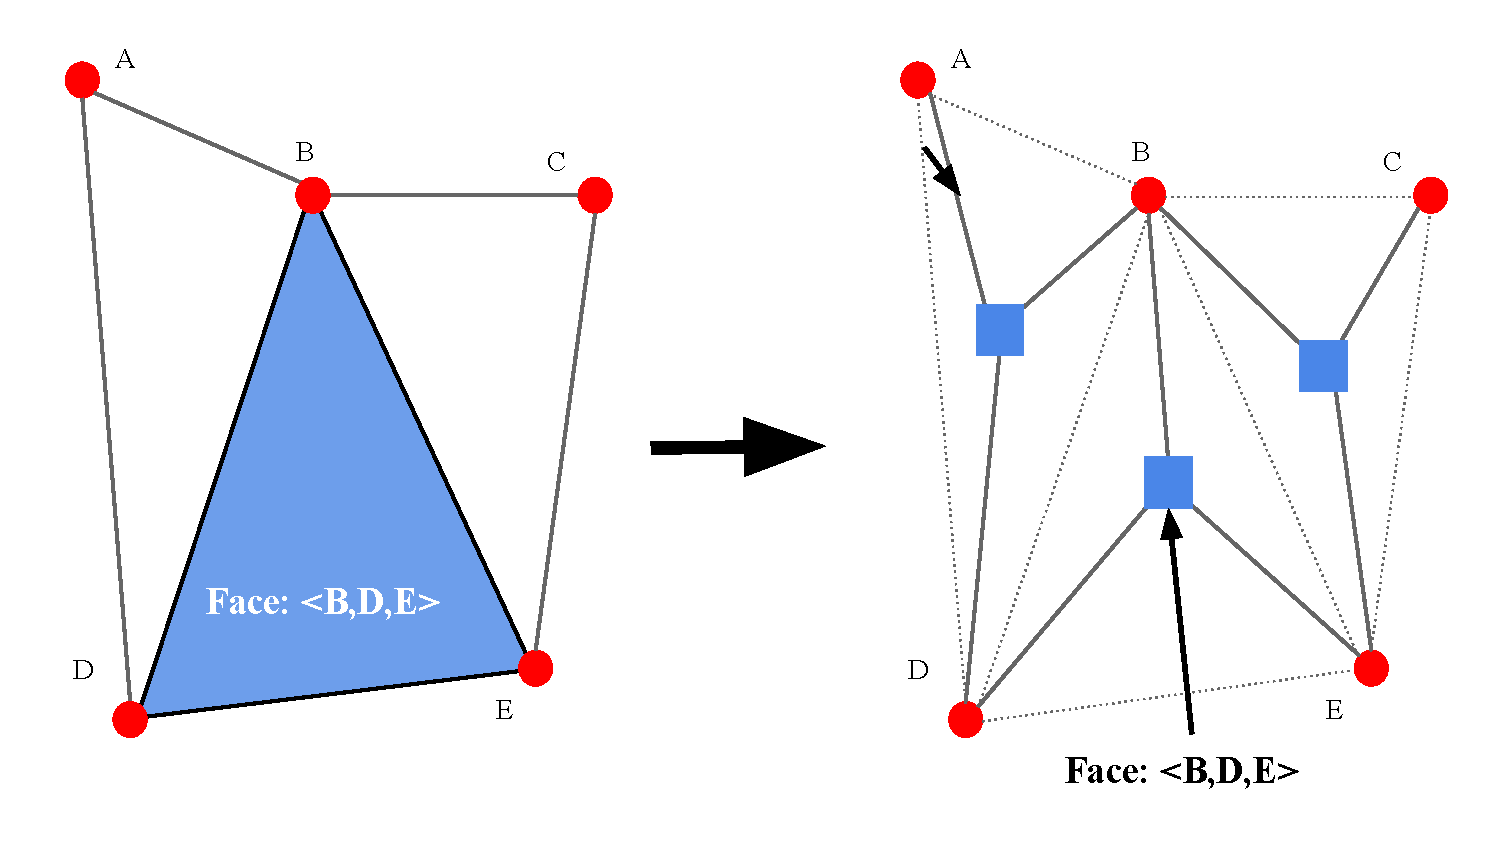
\includegraphics[width=4in]{hyperedge.pdf}
\caption{Graphs generated by the language Simit have hyperedges, an example
of which is in blue on the left.  Hyperedges are represented by different
\emph{types} of vertices in the resulting data-graph computation.
The square vertices in the figure represent hyperedges and have associated
per-hyperedge data.}
\label{fig:hyperedge}
\end{figure}

\begin{figure}[h]
\centering
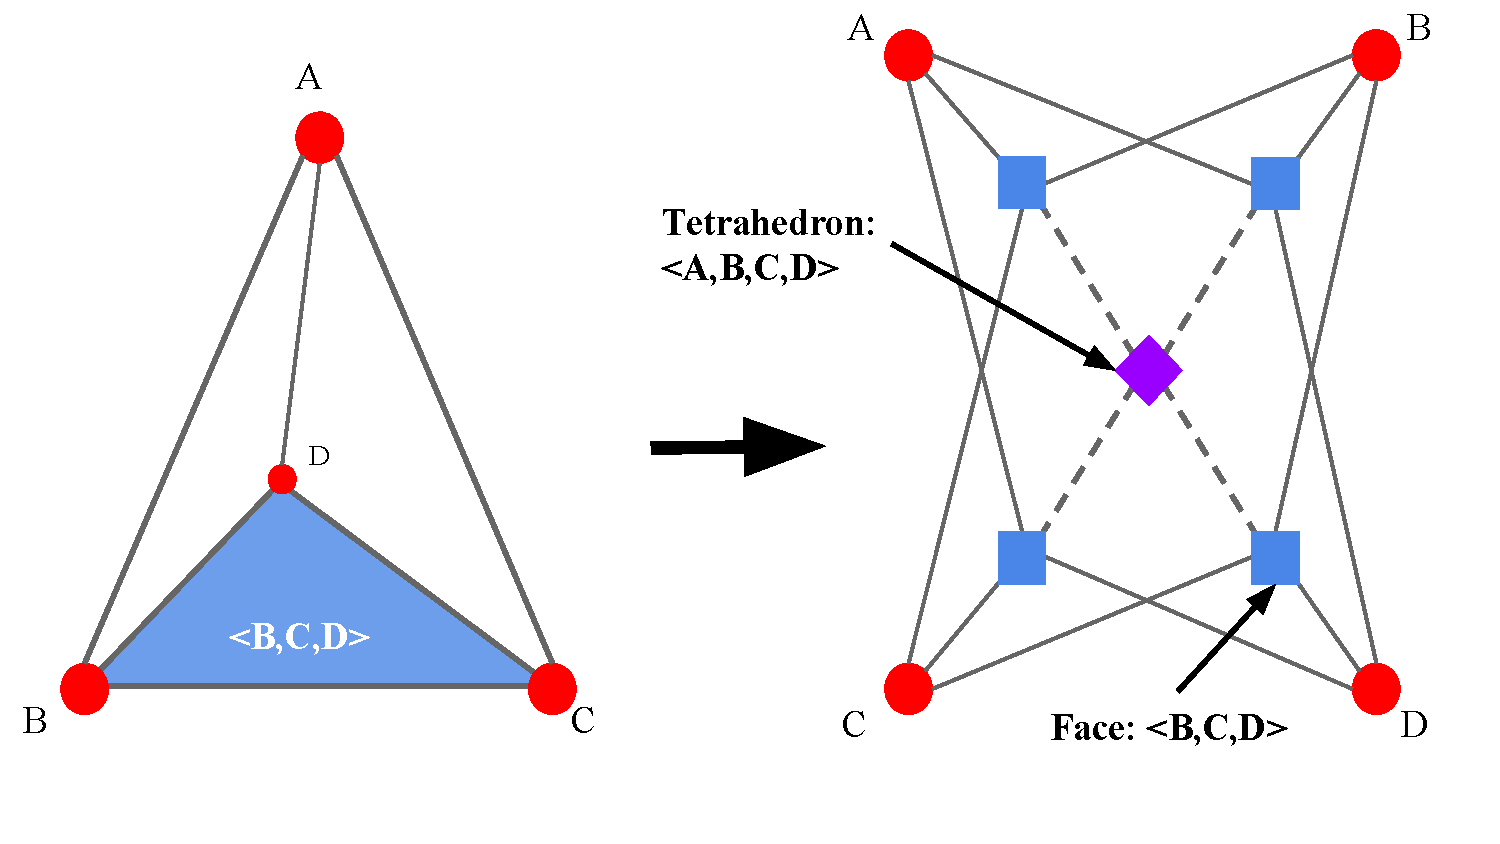
\includegraphics[width=4in]{tetrahedron.pdf}
\caption{Graphs generated by the language Simit have tetrahedrons,
as depicted on the left above.  A tetrahedron is composed of four
hyperedges (or \emph{faces}), an example
of which is in blue on the left.  Tetrahedra are represented by different
\emph{types} of vertices in the resulting data-graph computation.
The diamong vertex on the right represents a tetrahedron and is 
connected to its four constituent hyperedges.}
\label{fig:hyperedge}
\end{figure}



\subsection{Space-filling Curves}
		\begin{itemize}
		\item Quick qualitative overview of the cache behavior of our approach 
		\item Ditto for partitioning 
		\end{itemize}

\begin{figure}[h]
\centering
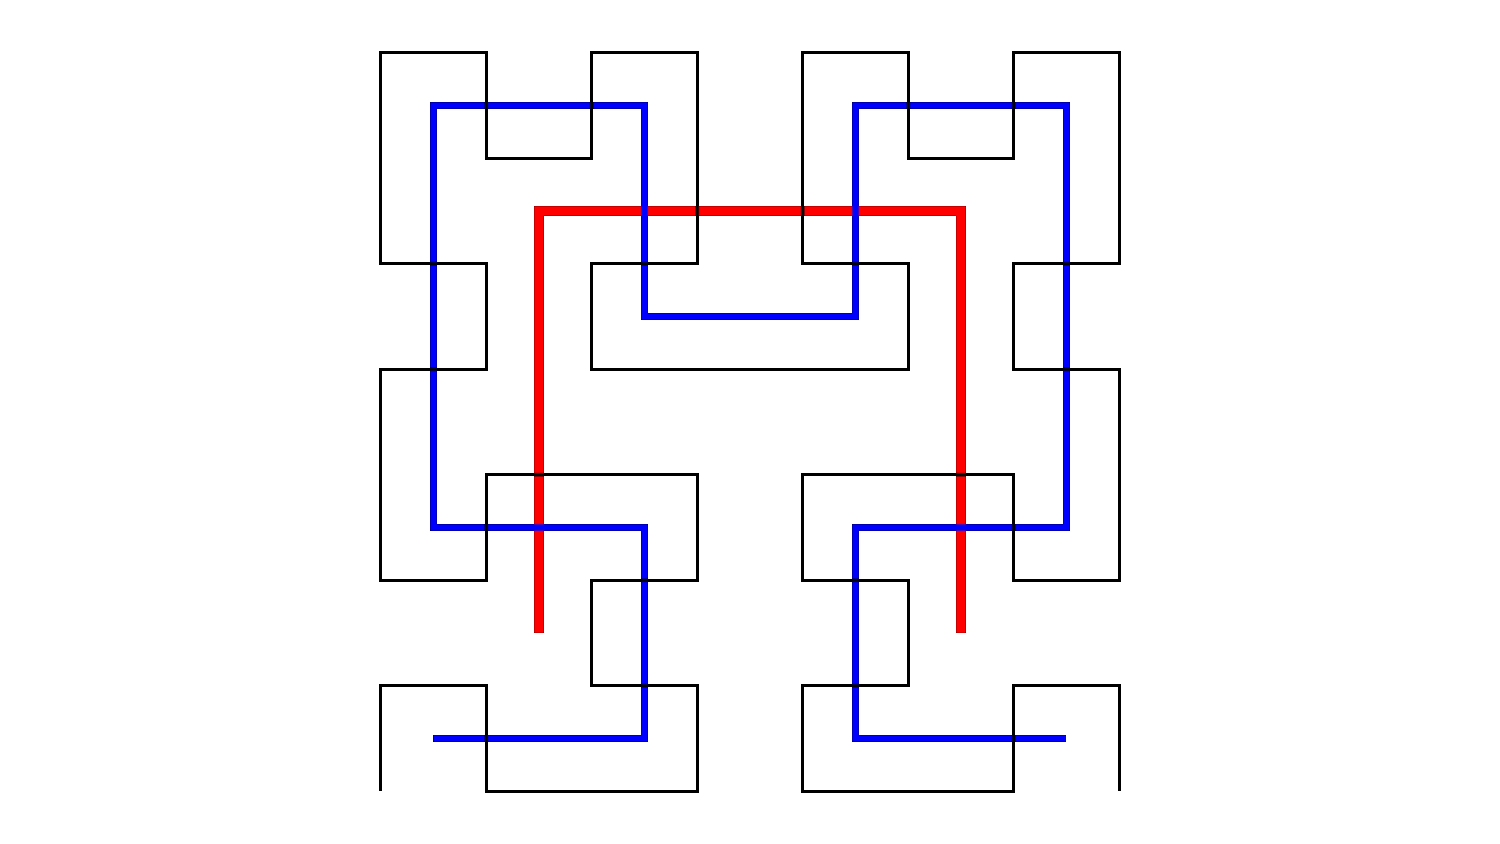
\includegraphics[width=4in,clip,trim=0 4cm 0 0]{2d_hilbert.pdf}
\caption{Three recursion levels of a 2-dimensional Hilbert space-filling
curve.  The red curve is the first recursion level and illustrates 
the basic 'U' shape.  The blue curve shows how each quadrant is
partitioned into four independent first-level Hilbert curves (up to 
rotations) of half the size in each dimension.  The black curve
illustrates the third recursion level.}
\label{fig:2d_hilbert}
\end{figure}


\subheading{Paper organization}



Old intro material:

In this work, we optimize a graph processing framework for a 
specific workload: physical mesh simulations. A mesh graph 
is embeddable in 3D space, and an example is shown in Figure 
1. Mesh graphs have the nice property that we can partition 
them into sets corresponding to arbitrary contiguous regions 
in physical space, and edges cross out of a particular set 
only from vertices near the boundaries of its physical region. 
Thus, the number of edges crossing out of a set is proportional 
to the surface area of its physical region, which is a fairly 
small quantity relative to the number of vertices, especially 
when the region has large volume.

Taking advantage of these properties, we use a novel method 
based on space-filling curves to split up an input mesh graph 
across machines to limit inter-machine communication. We then 
optimize performance on individual machines by evaluating a 
number of techniques for the scheduling of vertex updates that 
hit different points in the cache/TLB locality and parallelism 
design space. Some of our results yield insights for more 
general classes of graphs.

% Discussion of BSP vs. Gauss-Siedel?







% \subheading{Contributions}

% We anticipate contributing a new technique for and a well-engineered
% implementation of a cache-efficient data-graph computation using
% priority-dag scheduling.  In addition, our implementation will support
% extremely large simulations on distributed-memory clusters.  Both
% of these contributions are high-impact features for the customers
% of Simit, for which \proc{Prism} will be the new backend for multi-cores
% and clusters of multi-cores.  We have some initial exploratory code
% of priority functions (e.g. BFS depth, color).  

% \subheading{Task Breakdown}

% James and Predrag will extend \proc{Prism} to support data reshuffling
% based on a priority per vertex.  Initially, this will be a standalone
% utility that reads a graph file, reorders the vertices and writes out
% the shuffled file.  

% Will and Mohsen will engineer the MPI support for distributed memory,
% including support for distributed data loading.

% \subheading{Issues}

% We descoped our project to focus on being a good back-end for Simit, which
% works on graphs of physical simulations.  This means ditching the investigation
% of software prefetching and static assignment of vertices to processors.
% However, our new focus has allowed us to do something more elegant, essentially
% a cache-oblivious scheduling algorithm for data-graph computations on graphs
% of physical simulations.
